\documentclass[]{report}
\usepackage{graphicx}

%opening
\title{Working with MODFLOW}
\author{Roy Henson}

\begin{document}

\maketitle

\tableofcontents

\chapter{Introduction}
\section{Introduction}
Aquifers supply the water that is needed for drinking water and irrigation for much of the west and the United States. Making sure that the aquifers are clean and full is of great importance for everyone. With increasing development of the Boise area, the snake river basin aquifer saw a dramatic decrease in the aquifer level around the early 2000’s. When aquifers run low, aquifer recharge may be the best option to preserve it.
Aquifer recharge is taking water from damns, streams, or rivers, cleaning it, then pumping into the ground to recharge the local aquifer. There can be several problems that come with aquifer recharge and many ways to do it. The one that I will address is well, shaft, and borehole recharge. This is the type that is occurring currently in the Boise valley at the micron site. Some of the problems that can occur with aquifer recharge are, feasibility at a suggested site, optimal design of the system, optimization of managed aquifer recharge systems, quantify the recovery efficiency, and residence time of infiltrated water just to name a few. Most, if not all, of these issues can be modeled and solved with the modeling program called MODFLOW.

Modeling the flow of ground water is interesting to me because you can’t see the water physically. The only thing that can be monitored is water that is tested. As the groundwater moves it carries nutrients, ions, pollutants, and other water-soluble compounds. As these compounds are moved through the ground they are tested for through wells. From these compounds, we can see the flow of the water through the ground. Using a modeling program like MODFLOW allows engineers to better plan for difficulties that could arise but aren’t seen at the current moment of planning.

\chapter{Model Description}
\section{MODFLOW} 
MODFLOW is a modular program produced by the USGS in the 1980’s. It has gone through several revision and is still used today for many ground water applications. What makes MODFLOW modular is that there are different packages that can be added or subtracted from the main program for specific situations. It was originally marketed as a stereo system that you could plug in and tune different packages for different uses.

\begin{figure}[h]
	
	\centering
	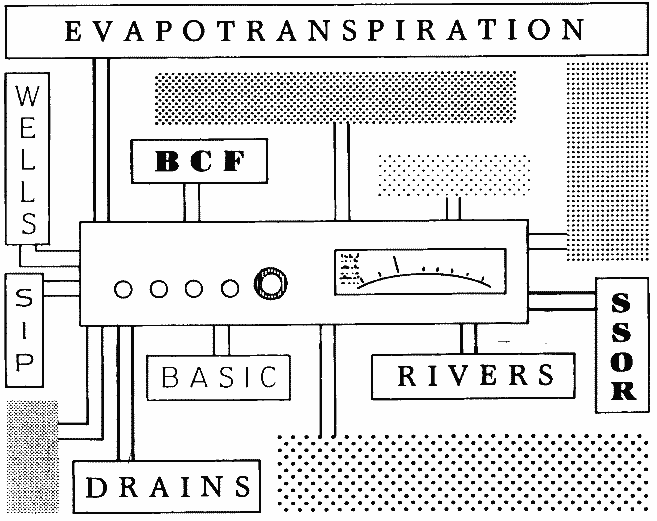
\includegraphics[width=0.7\linewidth]{../../../GitHub/Geos518/Project/images/fig_ref2}
	\caption{Cover image from McDonald \& Harbaugh (1983) which illustrates a computer surrounded by modules and arrays used by MODFLOW. This was said at the time to resemble a "component stereo system".}
	\label{Fig:1}
\end{figure}

\section{Language}
The model uses Fortran as its coding language. It started with Fortran ’66 and with updates moved to Fortran ’77, Fortran ’90 and Fortran. Recent versions of MODFLOW are compatible with packages that use C, python, and other popular coding languages. The current version is called MODFLOW 6 and was released on July 30, 2021.

\section{Equations}
The main part of the model uses this partial differential equation for a confined aquifer:
\begin{figure}[h]
	\centering
	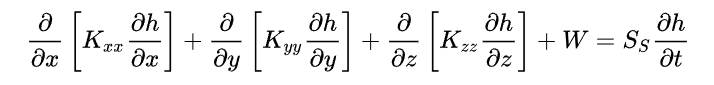
\includegraphics[width=0.7\linewidth]{../../../GitHub/Geos518/Project/equations/Equation_1}
\end{figure}
Where K are the values of hydraulic conductivity along the x, y, and z axes; h is the potentiometric lead; W is the volumetric head; S is the specific storage of the porous material; and t is for time.
There is also the finite difference form of the partial differential equation (shown below). This equation uses a discretized aquifer domain that uses rows, columns, and layers.
\begin{figure}[h]
	\centering
	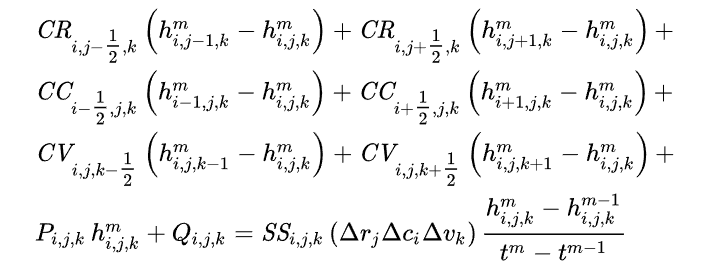
\includegraphics[width=0.7\linewidth]{../../../GitHub/Geos518/Project/equations/Equation_2}	
\end{figure}\\

Where $h^{m}_{i,j,k}$ is the hydraulic head at cell i,j,k at time step m; CV, CR, and CC are hydraulic conductance, or branch conductances between node i,j,k and a neighboring node; $P_{i,j,k}$ is the sum of the coefficients of head from the source and sink terms; $Q_{i,j,k}$ is the sum of constants from source and sink terms where $Q_{i,j,k}$\textless 0 is flow out of the ground water system and $Q_{i,j,k}$ \textgreater 0 is flow into the system; $SS_{i,j,k}$ is the specific storage; $\bigtriangleup r_{j}$ $\bigtriangleup c_{i}$ $\bigtriangleup v_{k}$ are the dimensions of cell i,j,k which when multiplied, represent the volume of the cell; and $t^{m}$ is the time at time step m. The equation can be formulated into a system of equations and is shown below.  

\begin{figure}[h]
	\centering
	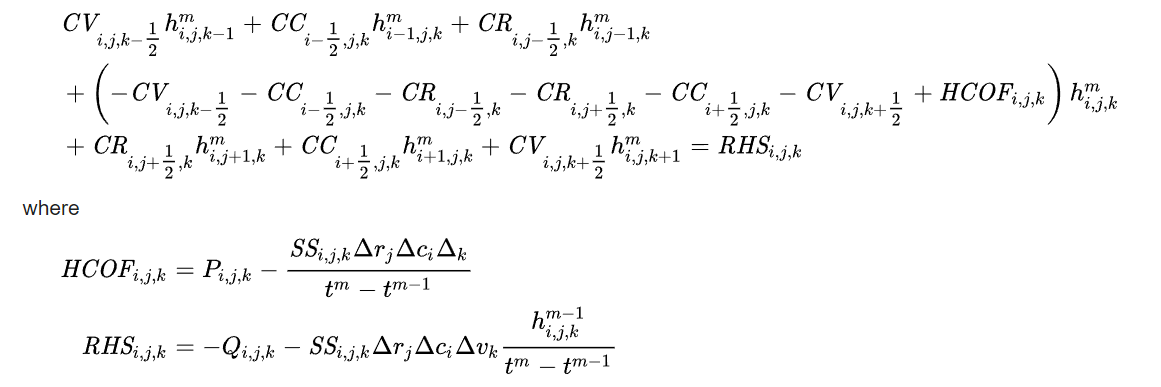
\includegraphics[width=1\linewidth]{../../../GitHub/Geos518/Project/equations/Equation_3}
\end{figure}


From these equations, we can define the parameters of the area that is going to worked with. From (Marston, 2012) “A parameter is a single value, which is given a name and determines the value of a variable in the finite-difference groundwater-flow equation at one or more model cells. Where parameters are used, the data value for a cell is either the parameter value or the calculated product of the parameter value and a cell multiplier, which could apply to many cells and can be described by using zones…Construction of the groundwater-flow model was accomplished by horizontally and vertically discretizing the hydraulic properties of the groundwater system, establishing model boundaries that depict conceptual hydrologic boundaries, and assigning model parameters to all stresses and aquifer properties.”\\
\section{Limitations}
There are some limitations of MODFLOW. It must be assumed that there is a constant density, dynamic viscosity and temperature throughout the aquifer that is being studied. Also, the model doesn’t work with non-orthogonal anisotropies, which I believe means that it doesn’t work well with water changing physical properties in a non-90 degree direction. \\
\section{Summary}
When MODFLOW was first created, the 3-D grid system was quite small, only 7 columns by 4 layers. Currently, the grids can be as large or as small as necessary. It started out as a model to track and monitor groundwater and aquifers and now with the new and upcoming packages that can work with MODFLOW, engineers can get a good representation of how ground water moves and any issues that might arise with aquifer recharge. \\




\chapter{Data Needs}

That data that is needed to run the model is the type of rock from each layer above, in and below the study area, the water level through out the entire study area, any wells present, ground elevations, any sources of sinks of water (which are not limited to wells drawing water from the aquifer, local rivers, and lakes/reservoirs that are feeding the aquifer, rain fall and evapotranspiration to name a few), the physical area of the study area, the hydraulic conductivity in the horizontal and vertical directions, if there is any current water flow in the aquifer and the estimated physical storage capacity of the study area. \\
It is also necessary to know of any fractures or faults in the study area because these could lead to unexpected sources or sinks to the model. They could make the model more difficult to run or lead to inaccurate results. Knowing that these are present can mean that a specific module is needed to run with the model to get accurate results. \\
There is also the need to know what the area will look like in the future. If you can figure out if there will be more wells or irrigation or is there will be more subdivision added you can add those to the model as well. \\
Collecting this information can take months to years to collect and is often dependent on previous studies of the bedrock for the area that is being modeled. Usually, the data comes from core samples which are taken from the area of study but can also come from dug trenches. \\
With MODFLOW having the capacity to add more modular packages to the main model, it makes sense that the more data you can acquire about the area of study the more modules will need to be added to the model and the more accurate the model will become. 

\chapter{Calibration}
The purpose of calibration for MODFLOW is to acquire a simulation that reasonably represents groundwater recharge, movement, discharge, and measured water levels in orders to predict the movement of recharge from the modeled/studied area and to estimate the additional storage capacity of underlying bedrock and the long-term discharge to local rivers or to other bodies of water. \\
Depending on the situation and study area all the variables that would be needed to run MODFLOW could be adjusted by calibration. There are some variables have a higher chance of needed calibration. They are hydraulic conductivity in the vertical and horizontal direction, anisotropy, specific yield, specific storage, natural recharge as infiltration of precipitation, reservoir recharge and any other sources or sinks that occur.  \\
Sensitivity analysis need to be done to determine which variables provided by the observations need to be eliminated because they are too sensitive, and to know which parameters can be combined or divided. 
Nonlinear Regression can be used to produce simulations that fit the observations by adjusting parameter values to reduce the least-squares objective function by using weighted residuals. \\
After a sensitivity analysis and nonlinear regression, the parameters are adjusted to their final values for the model. Some of the reasons they are adjusted are that observations do not always provide enough information to estimate it correctly, sometimes flux observations have more uncertainty than head observations, parameters can change from before and after recharge, and the bedrock that the aquifer is in may need to be broken down so that it uses more than one variable/parameter for the study area/aquifer area. 

\chapter{Numerical Experiment Design}
\section{Introduction}
\subsection{Introduction}
The purpose of the report is to “describe the groundwater hydrology of the Hurricane Bench area and to present the construction, calibration, and projected results of a numeri¬cal simulation of the groundwater system in the Hurricane Bench area, including recharge from Sand Hollow Reservoir”. The report covers the aquifer, the groundwater, the groundwater budget, and the model they used to track the aquifer and water movement over time. The report was done by Marston, T., and V. Heilweil for USGS.\\
\begin{figure}[h]
	\centering
	\begin{minipage}{0.4\textwidth}
		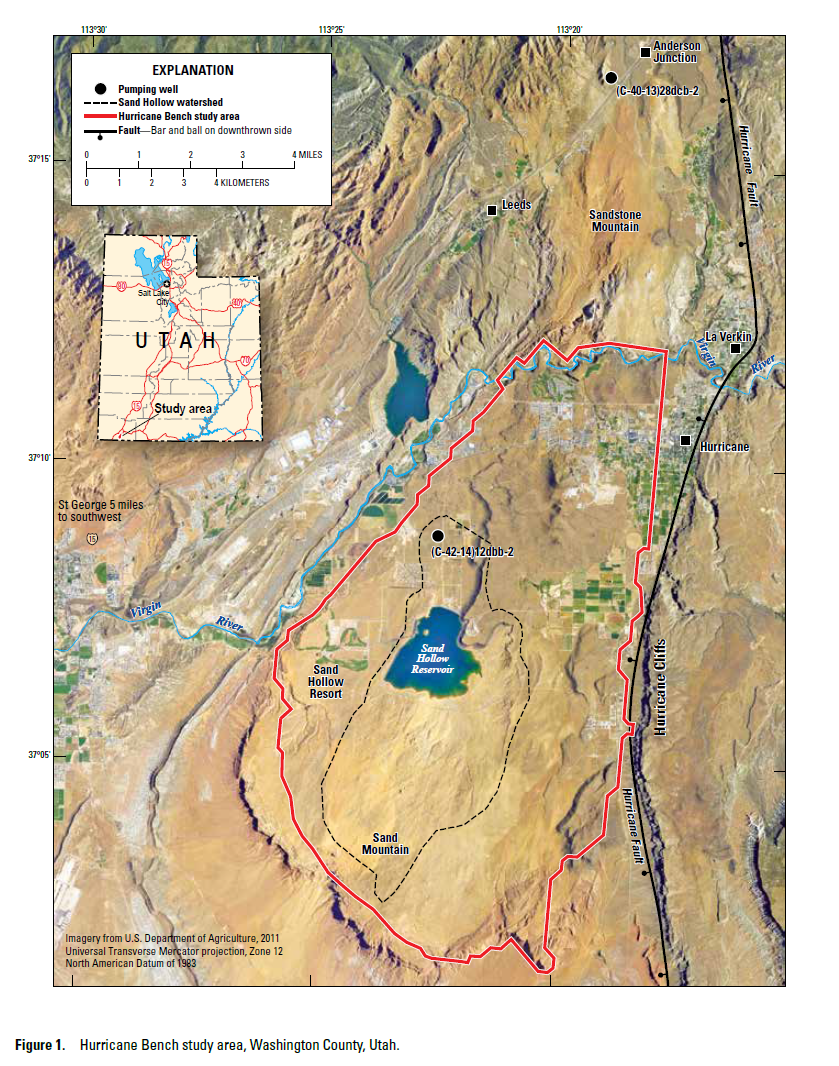
\includegraphics[width=1.0\linewidth]{../../../GitHub/Geos518/Project/images/Fig_1}
	\end{minipage}
	\hfill
	\begin{minipage}{0.4\textwidth}
		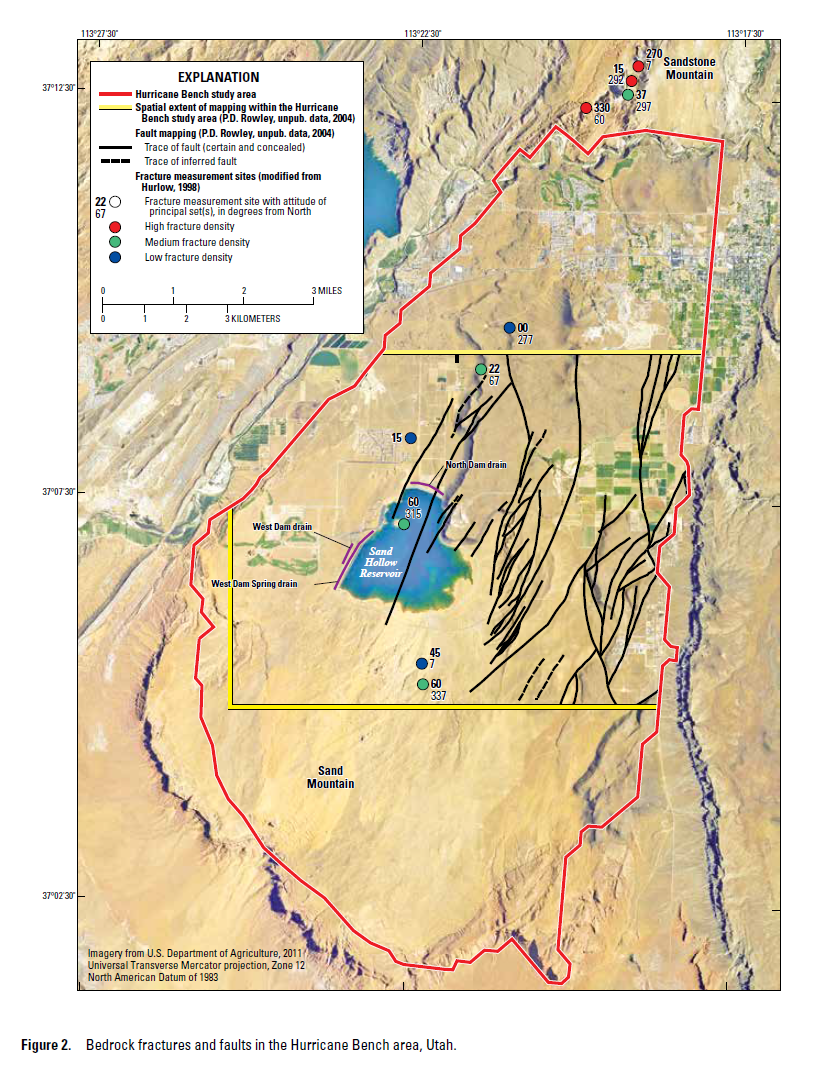
\includegraphics[width=1.0\linewidth]{../../../GitHub/Geos518/Project/images/Fig_2}...
	\end{minipage}
\end{figure}

\subsection{Aquifer}
The Sand Hollow Reservoir has a thin layer of soil followed by Navajo sandstone then goes on to be Kayenta formation. The lower boundary is a layer of siltstone underneath the Kayenta formation. The water from the reservoir flows through the sandstone and into the Kayenta formation where then it can travel to the virgin river.\\
\subsection{Groundwater}
The groundwater around the Sand Hollow Reservoir now moves in all directions away from the reservoir. Before the reservoir was constructed, the water mostly flowed north, towards the Virgin River. The water is boarded by a fault to the east that likely restricts the flow of water and a border on the west side that has low permeability rocks. As the wells in that area have been monitored, they saw a significant decrease in the water table around 1995 assumed to be due to increased well usage for irrigation. Since the reservoir was created in 2002, it has caused an increase in the groundwater table around the reservoir.\\
\begin{figure}[h]
	\centering
	\begin{minipage}{0.4\textwidth}
		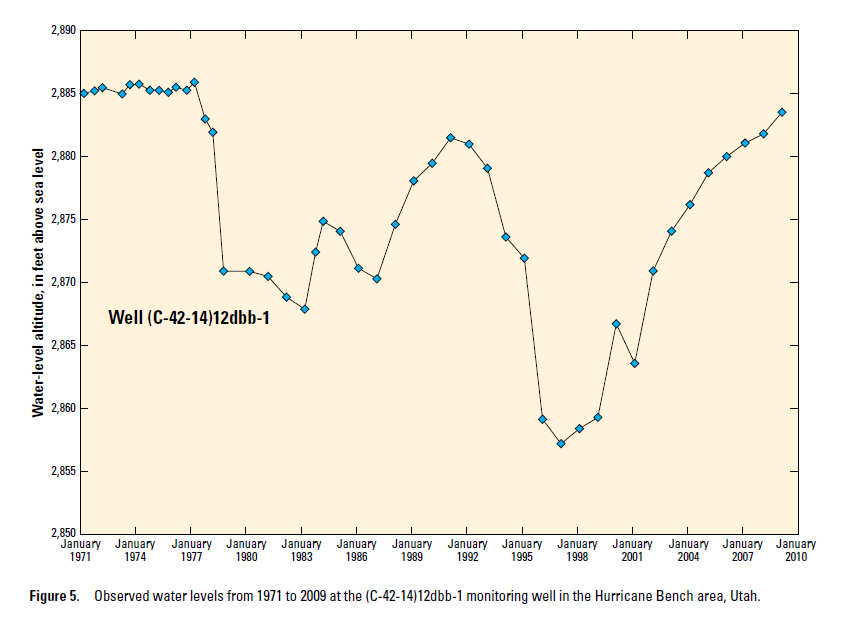
\includegraphics[width=1.3\linewidth]{../../../GitHub/Geos518/Project/images/Fig_5}
	\end{minipage}
	\hfill
	\begin{minipage}{0.4\textwidth}
		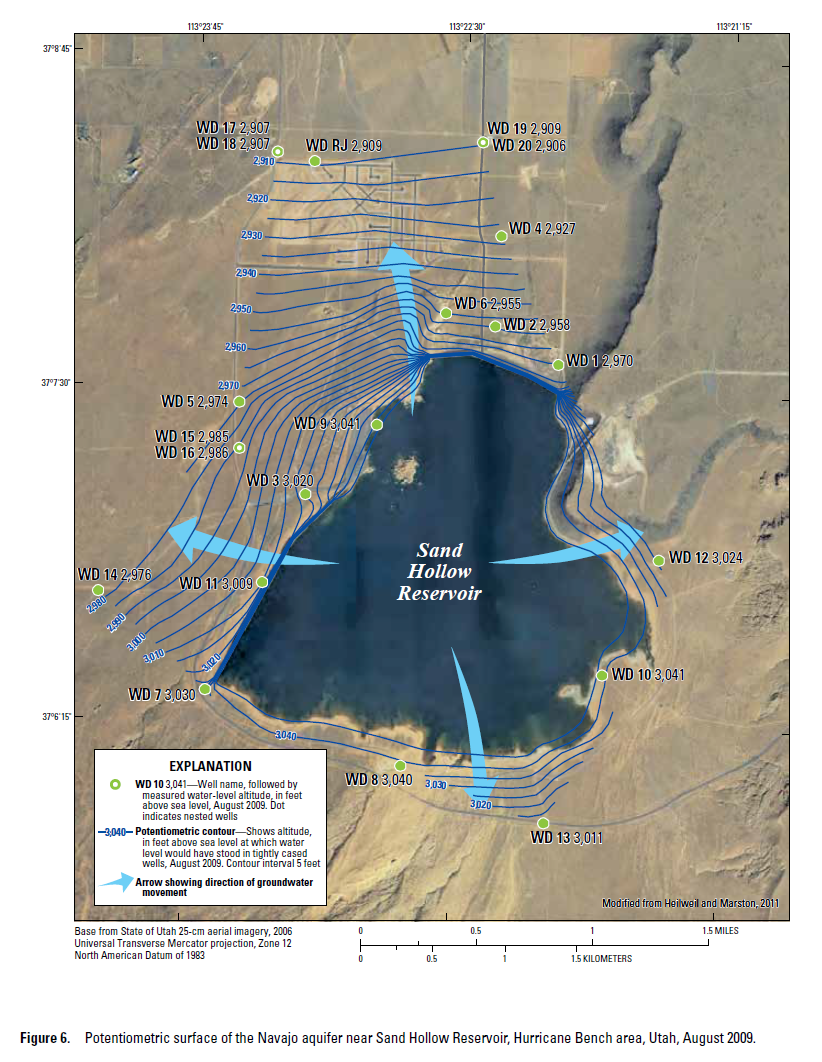
\includegraphics[width=1.1\linewidth]{../../../GitHub/Geos518/Project/images/Fig_6}
	\end{minipage}
\end{figure}
 \subsection{Groundwater Budget}
Ground water budget The only groundwater recharge before the Sand Hollow Reservoir was natural infiltration of rainwater. Since the reservoir has been built, it now contributes most of the water to the groundwater system. There could be several things that could be slowing or stopping water from reaching the groundwater system some of which could be declining hydraulic gradients, the accumulation of silt and biofilms, and gas clogging.\\
  
There are 2 ways in which discharge of water from the Sand Hollow Reservoir system, seepage into the virgin river and draws from wells. Many of the wells are for irrigation and used between June – August. There are 2 city wells used for municipal water. After the completion of the reservoir, there were 2 drainage ditches built that allows for shallow groundwater that are next to the reservoir that add to the total discharge.\\
\section{Model}
\subsection{Model}
A model was constructed using MODFLOW to simulate managed aquifer recharge from Sand Hollow Reservoir and the subsequent movement of groundwater through the Hurricane Beach area.

\subsection{Construction}
Construction of the model was done by approximating the hydraulic properties of the groundwater system, establishing model boundaries based on the conceptual boundaries, and assigning parameters to all stresses and aquifer properties (except the immediate reservoir area).
\begin{figure}[h]
	\centering
	\begin{minipage}{0.4\textwidth}
		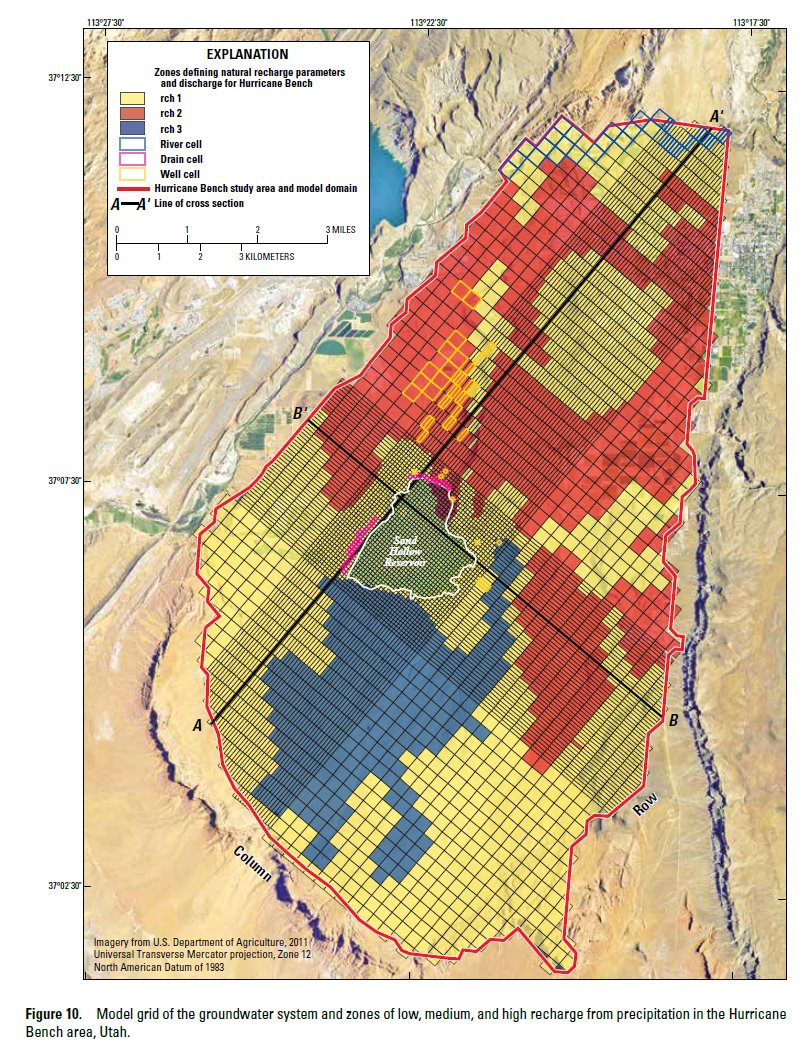
\includegraphics[width=1.1\linewidth]{../../../GitHub/Geos518/Project/images/Fig_10}
	\end{minipage}
	\hfill
	\begin{minipage}{0.4\textwidth}
		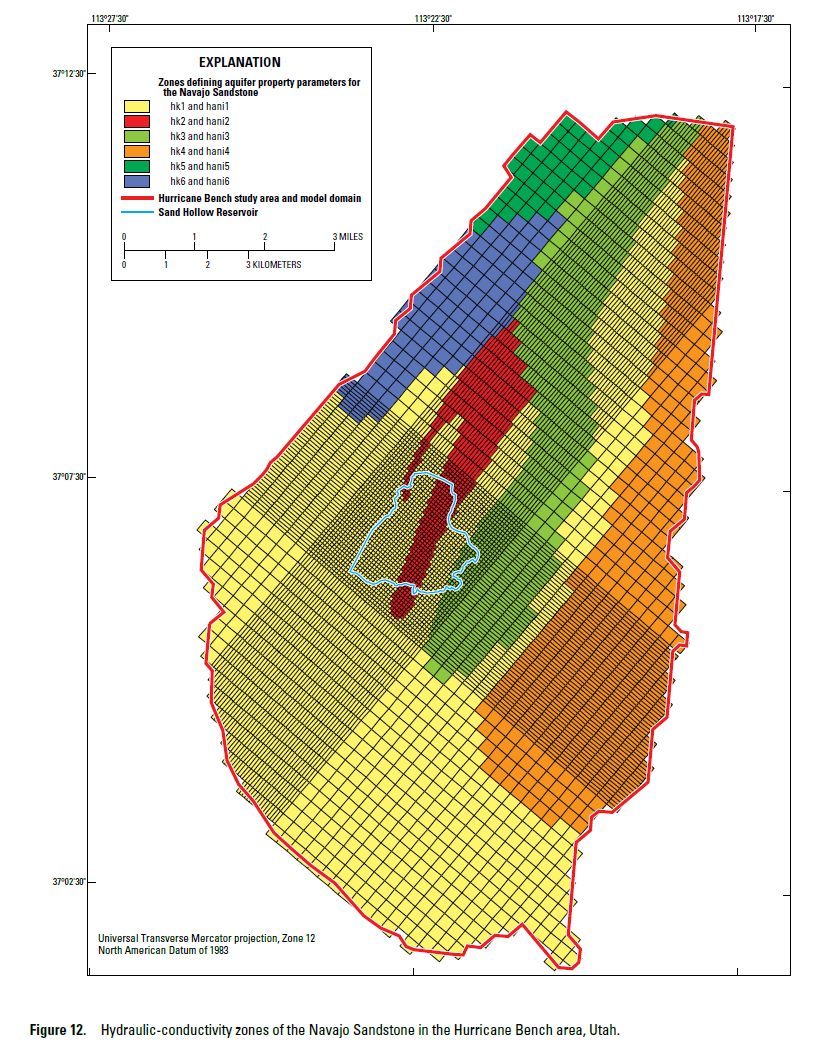
\includegraphics[width=1.1\linewidth]{../../../GitHub/Geos518/Project/images/Fig_12}
	\end{minipage}
\end{figure}
\begin{figure}[h]
	\centering
	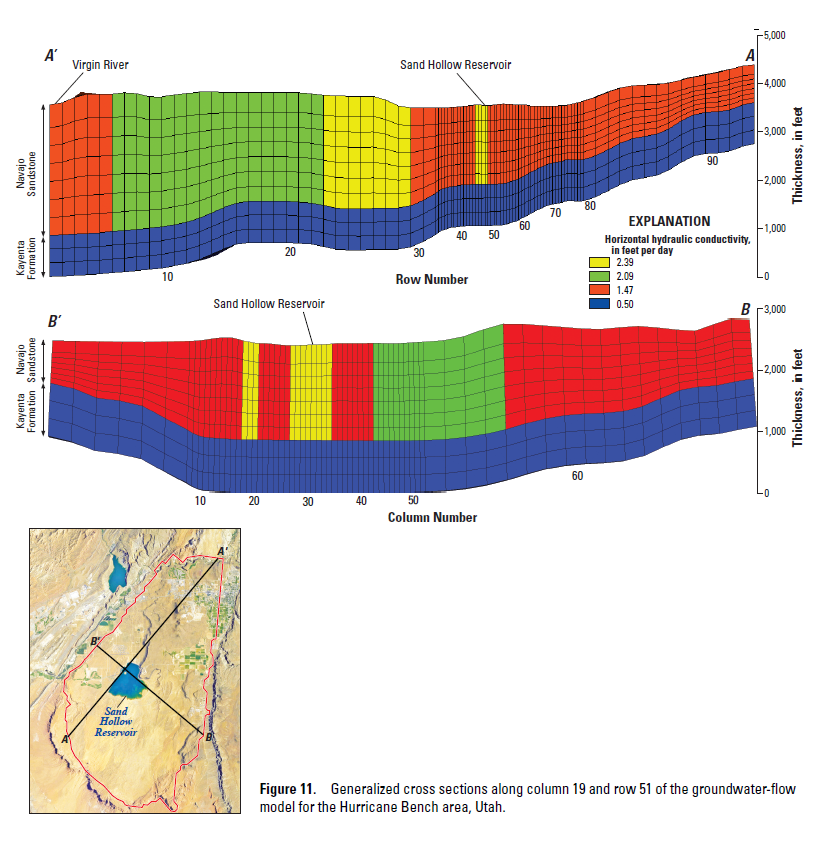
\includegraphics[width=1.1\linewidth]{../../../GitHub/Geos518/Project/images/Fig_11}
\end{figure}
\subsection{Calibration}
A calibration of the parameters used in the model was done to make the model a closer approximation. That calibration was done in a manner that was like the explanation of calibration stated previously in this report.
\subsection{Accuracy}
There was a large amount of discharge, recharge and water level provided with the Sand Hollow Reservoir area that proved to be relatively accurate. There was a low amount of data for the water-level measurements and aquifer stresses away from the reservoir. This caused uncertainty in hydraulic properties and fluxes which in turn caused combination of recharge, discharge, and aquifer properties to yield similar or improved results. Observations can only provide so much information for some parameters which made it difficult to assess how well they were estimated in the model.
\begin{figure}[h]
	\centering
	\begin{minipage}{0.4\textwidth}
		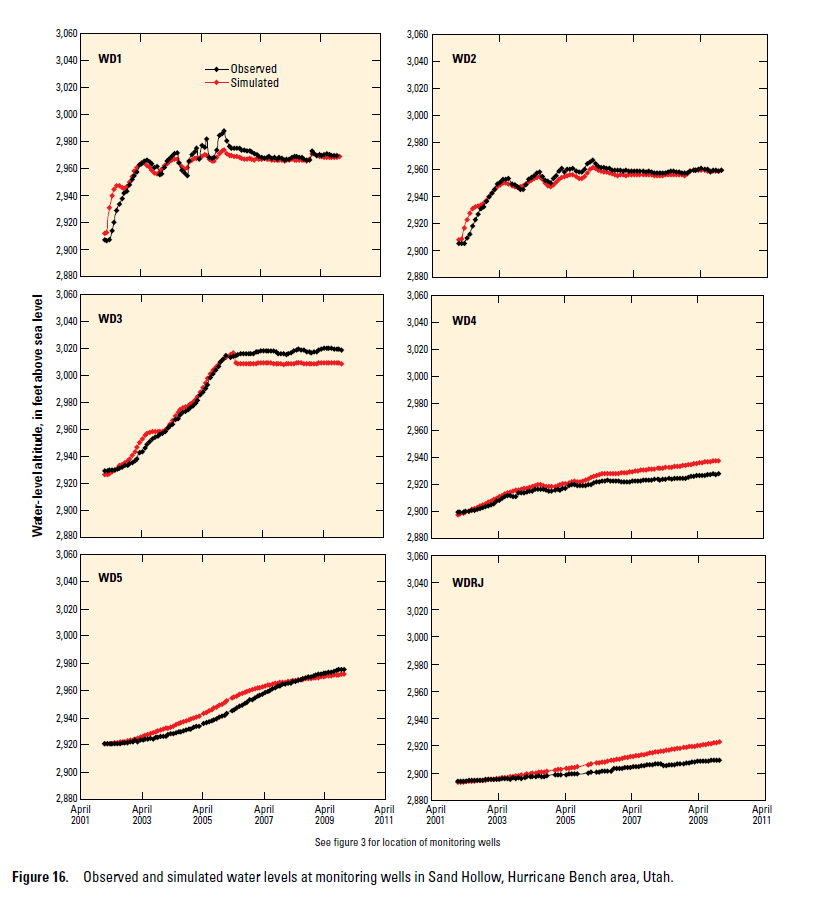
\includegraphics[width=1.1\linewidth]{../../../GitHub/Geos518/Project/images/Fig_16a}
	\end{minipage}
	\hfill
	\begin{minipage}{0.4\textwidth}
		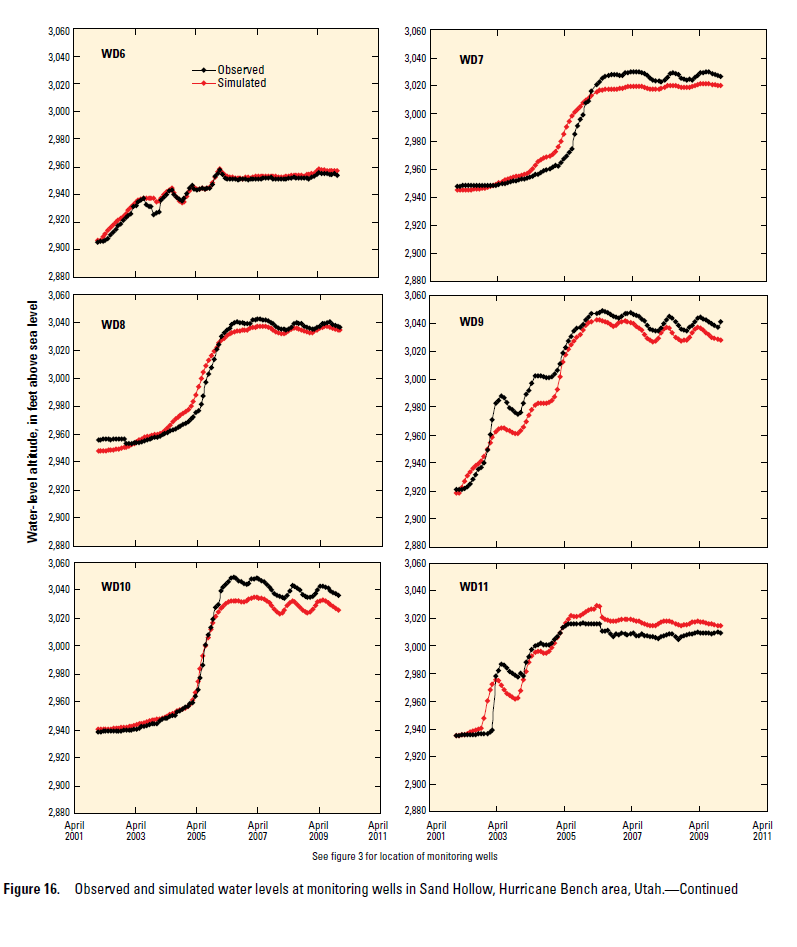
\includegraphics[width=1.1\linewidth]{../../../GitHub/Geos518/Project/images/Fig_16b}
	\end{minipage}
\end{figure} 
\subsection{Projections}
The model correctly predicted what happened in the past when the reservoir was created and how the monitoring wells reacted. That gives confidence that the future projections will be correct as well. In Figure 19 it shows the long-term flow of the groundwater flow from the Sand Hollow reservoir to the Virgin River.
\subsection{Limitations}
Limitations on the model are uncertainties in the hydraulic conductivity in areas that are far away from the reservoir, discharge assumptions of the Virgin River, assuming that the porous media was continuous in a fractured dual permeability aquifer system, assuming that the storage properties were continuous, not including a possibility for groundwater upwelling from the underneath, and simulations using of shallow drains.

\section{Summary}
The purpose of the report was to present a numerical simulation of groundwater movement in the Hurricane Bench area, including aquifer recharge. From the data presented and used, the model was with in an acceptable margin of error and fulfilled its purpose. MODFLOW-2005 was used with the necessary modules
\begin{figure}[h]
	\centering
	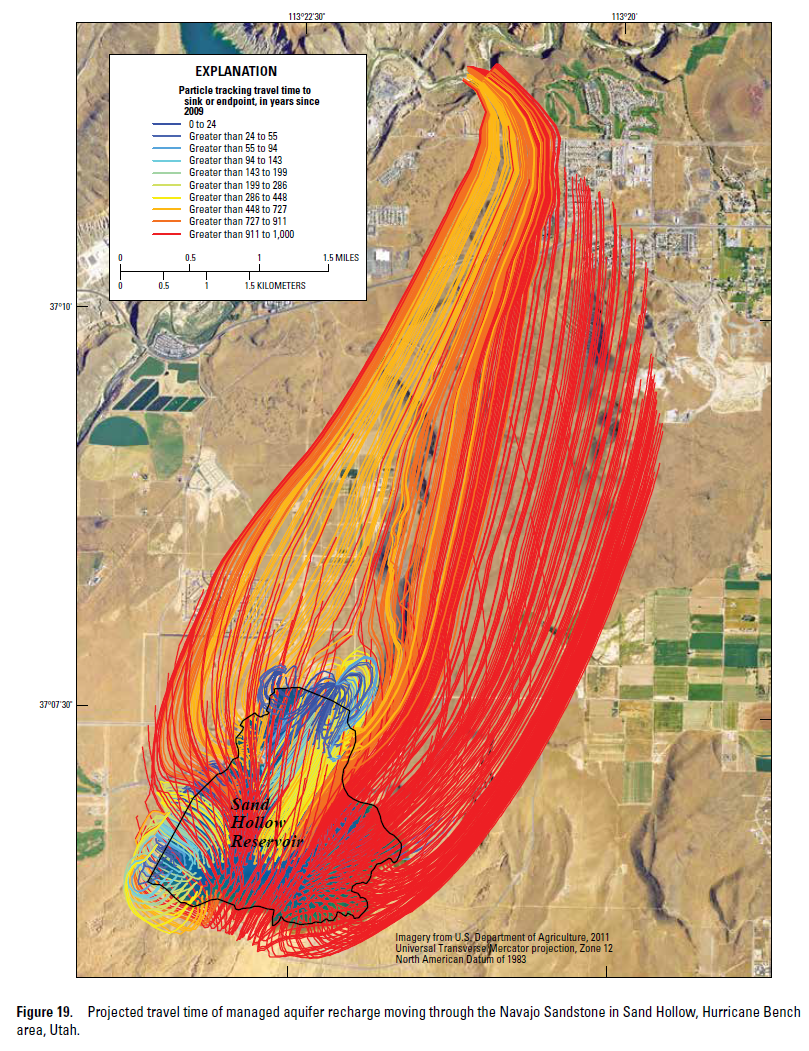
\includegraphics[width=1.1\linewidth]{../../../GitHub/Geos518/Project/images/Fig_19}
\end{figure}






\chapter{References}
Harbaugh, A. (2021), MODFLOW-2005, The U.S. Geological Survey Modular Ground-Water Model—the Ground-Water Flow Process, Pubs.usgs.gov. Available from: https://pubs.usgs.gov/tm/2005/tm6A16/PDF/TM6A16.pdf (Accessed 15 December 2021)\\

Marston, T., and V. Heilweil (2012), Numerical simulation of groundwater movement and managed aquifer recharge from Sand Hollow Reservoir, Hurricane Bench area, Washington County, Utah, USGS.gov. Available from: https://pubs.usgs.gov/sir/2012/5236/pdf/sir20125236.pdf (Accessed 15 December 2021)\\

McDonald, M., and A. Harbaugh (2003), The History of MODFLOW, Ground Water, 41(2), 280-283, doi:10.1111/j.1745-6584.2003.tb02591.x.\\

McDonald, M., and A. Harbaugh (1984), A modular three-dimensional finite-difference ground-water flow model, Open-File Report, doi:10.3133/ofr83875.\\

Ringleb, J., J. Sallwey, and C. Stefan (2016), Assessment of Managed Aquifer Recharge through Modeling—A Review, Water, 8(12), 579, doi:10.3390/w8120579.\\
\end{document}
